\documentclass[12pt]{article}
\usepackage[utf8x]{inputenc}
\usepackage{amsmath}
\usepackage{graphicx}
\graphicspath{{Images/}}
\usepackage[colorinlistoftodos]{todonotes}
\usepackage{hyperref}

\begin{document}
\begin{titlepage}
\newcommand{\HRule}{\rule{\linewidth}{0.1mm}} 
\center % Center everything on the page
 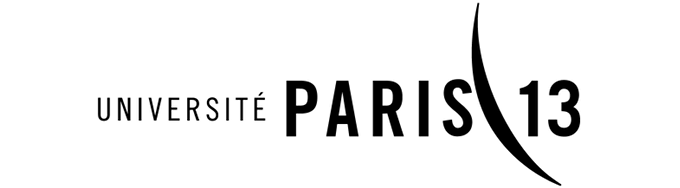
\includegraphics[scale=0.5]{image.png}% \\[0.5cm] % 



\textsc{\Large Institut Galilée Université Paris 13 Villetaneuse}\\[0.5cm] % heading course name
\textsc{\large 2018-2019 }\\[0.5cm] % Minor heading


\HRule \\[0.4cm]
{ \huge \bfseries Projet LEE \\

 \large feuille de route modulable (Accueil international) }\\[0.1cm]
 
\HRule \\[1.5cm]


\begin{minipage}{0.4\textwidth}
\begin{flushleft} \large

\emph{Réalisé par :}\\
 MAHDOUANI  \textsc Yassine\\PLS.  % Enter Your name and T.No.
\end{flushleft}


\begin{flushleft} \large

\emph{Enseignant:}\\
M. Pierre \textsc{Boudes}\\ 
\end{flushleft}
\end{minipage}
\end{titlepage}



\newpage

% Do not edit the below sections, enter all details in respective chapters
% Add the images/screen-shorts to the image folder and insert them in the respective chapters

\section{Introduction}

% Introduction

% Please delete the below lines and enter details for this assignment/homework
\paragraph{}

Le projet consiste le creation de feuille de route pour l’arrivée en France des future étudiant.es, chercheurs et chercheuses de l’Université de Paris 13, c’est la création d’un format de donnée permettant le stockage des feuilles de routes sous une forme structurée .





\section{Pourquoi Feuille de route ?}
Une feuille de route peut prendre plusieurs significations en fonction du contexte :

 Dans nos cas Feuille de route est couramment employée pour désigner les grandes lignes, et surtout les étapes à suivre .


Dans nos Feuilles de routes , on stocke des informations personnalisées et un calendrier étape par étape qui nous indique toutes les démarches à effectuer avant  de venir en France.
 
 Quelles démarches avant votre arrivée en France ?

Visa - assurance maladie - banque -  titre de séjour
Vos démarches en fonction de votre situation.



\section{Environnement}
% Results
% Please delete the below lines and enter details for this assignment/homework


Le projet est crée en Java 
\begin{itemize}

    \item . Eclipse IDE for Java Developers
    \item Version: 2018-12 (4.10.0)
    \item Build id: 20181214-0600
    \item JRE Sytem Library [JavaSE-10]
    
    

\end{itemize}

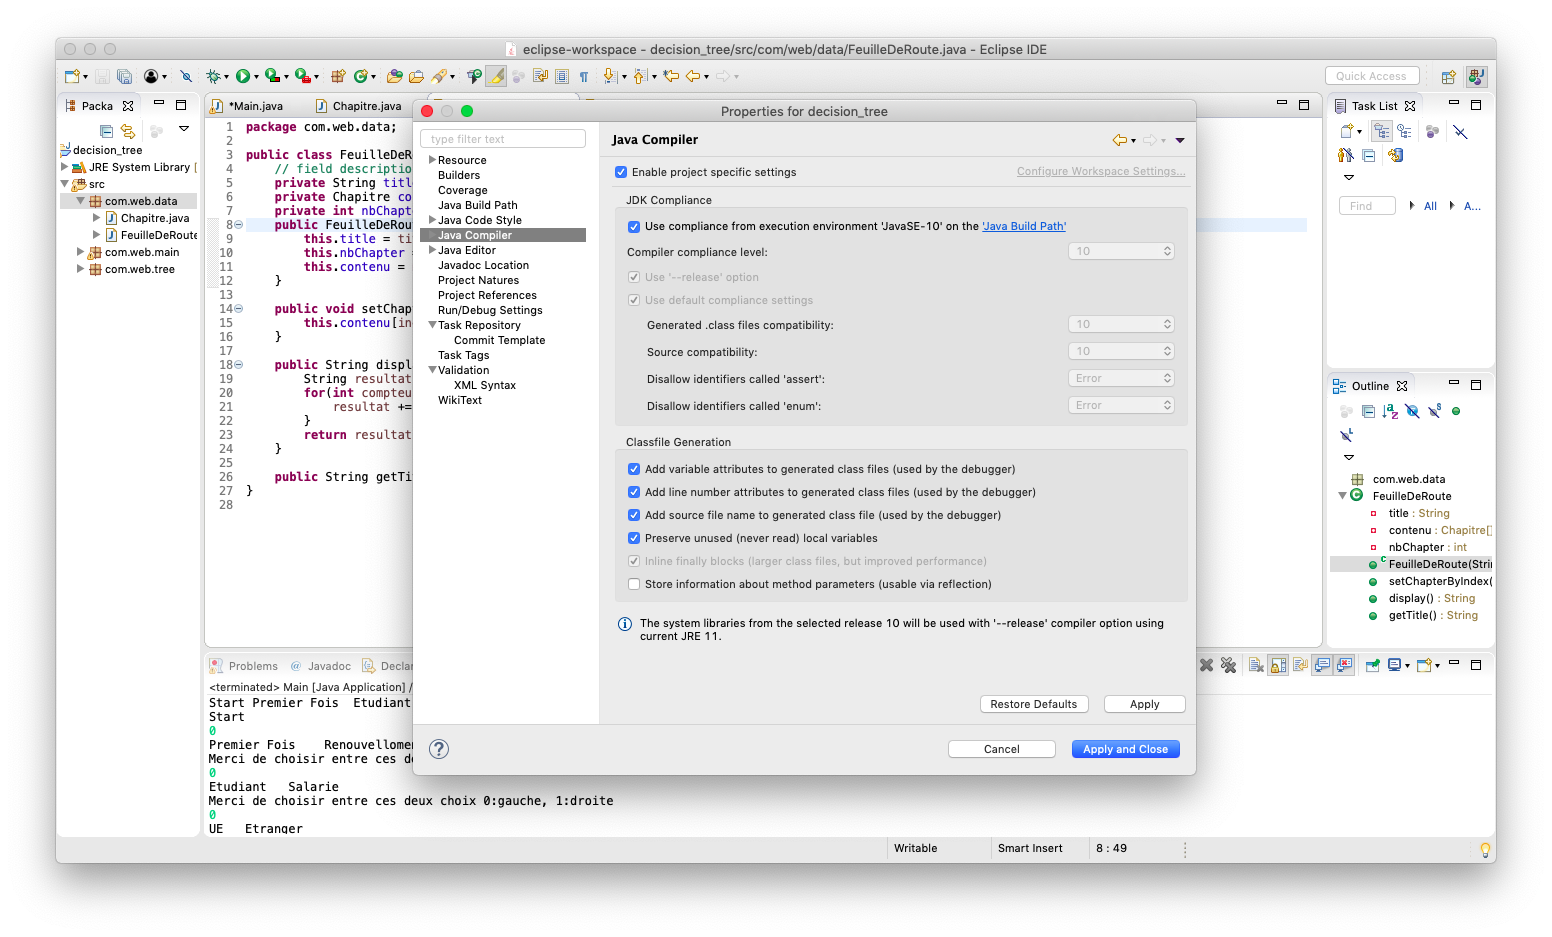
\includegraphics[scale=0.3]{env.png}% \\[0.5cm] % 

\section{Développement}
% Discussions & Conclusion
% Please delete the below lines and enter details for this assignment/homework
    Pour crée mes Feuilles de routes j’ai basé sur Package de l’arbre de
    Décision com.web.tree dans mon projet Accueil international .

\begin{enumerate}

\item Package: com.web.tree 
\begin{itemize}
\item Class Tree.java   : Contient les fonctions et les méthodes de creation et manipilation de notre arbre de décision .
Danns notre cas c'est une arbre de décision binaire avec quatre level inspire de l'exemple d'accueil international de Paris Saclay .


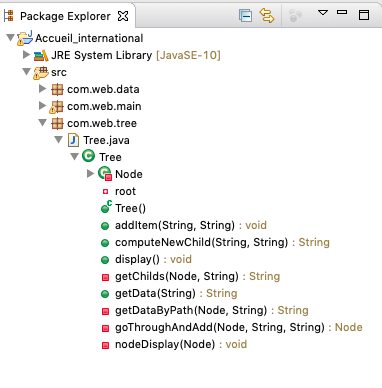
\includegraphics[scale=0.6]{Images/ad.png}

   
\end{itemize}


\item Package: com.web.data

\begin{itemize}
\item Class Chapitre.java : Stucture de base de notre fuille de route
\\Titre : Titre de Chaque Chapitre exemple Logement, Inscription .
\\ Contenu : Déscription de Chapitre .
\\DElais : délais a respecter pour le démarche adminstrative .

\item Class FeuilleDeRoute.java  :  Creation et affichage de feuille de route
selon l'index (index c'est le nombre des chapitres dans une feuille de route selon chaque cas ) .
\\

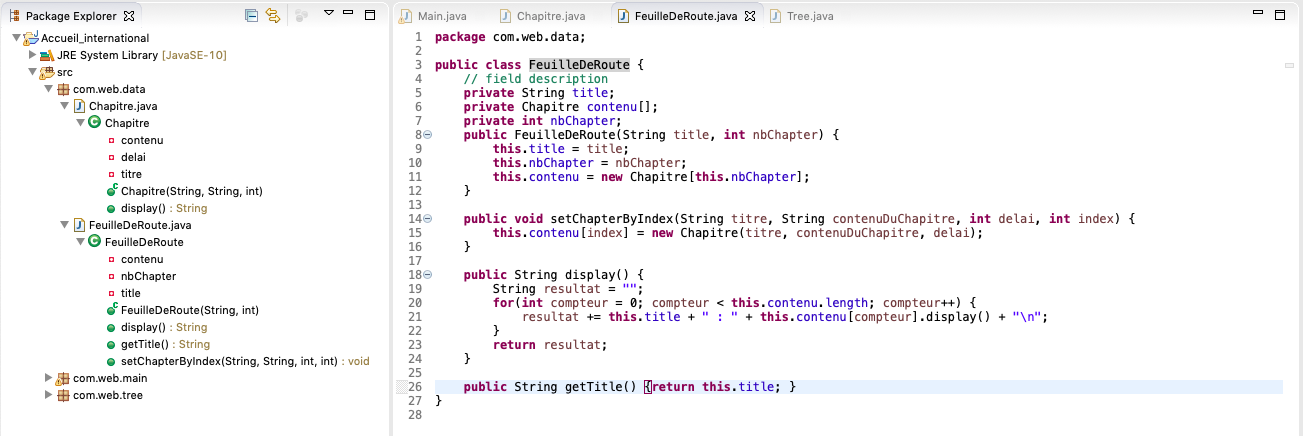
\includegraphics[scale=0.3]{Images/fdr.png}



   
\end{itemize}

\item Package: com.web.main  : Programme Principale 


 public static void main(String agrs[])
\\ Tous les fonctions de cration et affichage d'arbre de décisions et feuille de route .
\\Creation des feuille de route selon les feuille de notre arbre de décision.


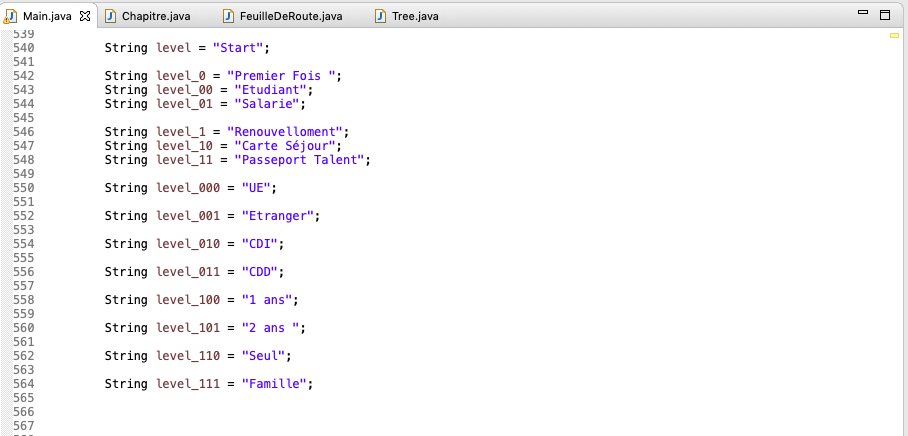
\includegraphics[scale=0.3]{Images/main.png}



   



\end{enumerate}



\section{Execution}
%
% Please attach the MATLAB or MULTISIM files (finial version) with this report
% Please delete the below lines and enter details for this assignment/homework
 L'execution de Main sert à exucuter l'arbre de décision et demander de l'utilisateur chaque  fois à choisir une option j'usqu'au validation de a choix et l'obtention de chemin final .\\
 \\(PATH: chemin binaire finale dans l'arbre) et selon ce Path on appelle une feuille de route déja crée automatiquement selon ce choix .\\
 
 BufferedWriter sert a crée les feuilles en format .txt avec ensuit le stocker selon une forme structurée .pdf \\
 
 exemple de feuille de route dans les deux format structurée texte et pdf .
 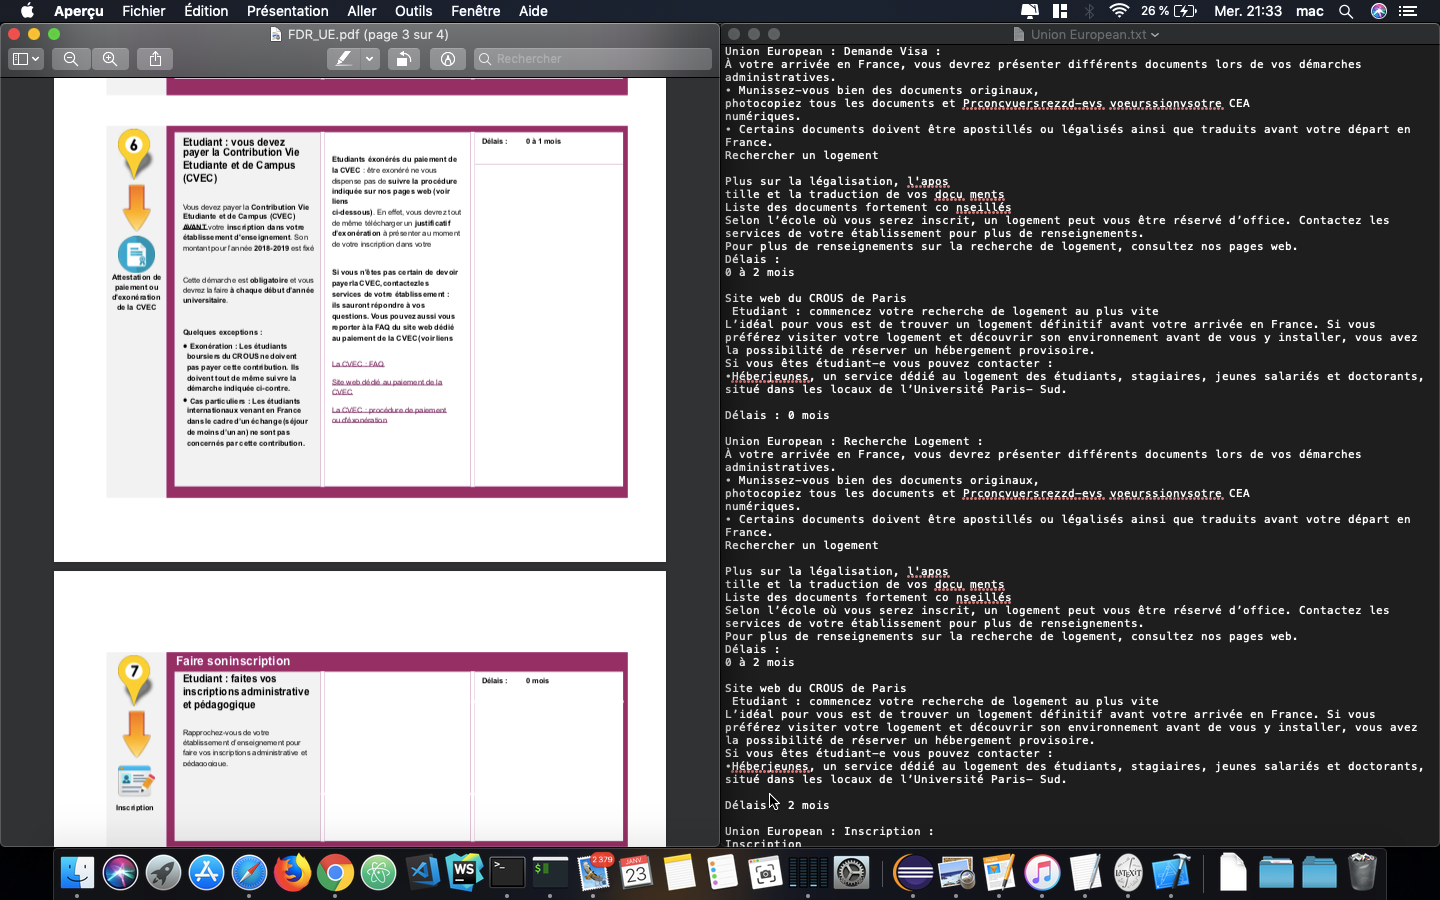
\includegraphics[scale=0.3]{Images/resultat.png}\\
 
 
\textbf{ Remarque :Il faut preciser le chemin où voulai avoir les feuilles de routes sur votre machine .}\\


\textbf{ lien de Gitlab : https://github.com/yassmhd/LEE2019 }







%---------------------------------------------------------------------------------
%	Example SECTION (Remove this section to finalize the report.


------------------------------------------------------


\end{document}


% Note: Again, you don’t need to answer just the above questions. They are being provided to give you a flavor of what is required for each section. Use your judgment and initiative to add or subtract based on the specific homework. You can add any other conclusion or discuss any other aspect of your effort that you think it is important to highlight.
